%----------
\section{Sorption and decay}

\subsection{Single component}

\subsubsection{Definition}

The aim of this example is to simulate the solute transport in an aquifer by convection with the influence of retardation as a result of sorption. Additionally, the transported mass will be degraded. The calculation area and boundary conditions are the same as described in chapter \ref{sec:decay}.

The following simplifications are assumed: (1) linear sorption, decay of components (2) homogeneous aquifer, saturated, stationary flow (Fig. \ref{fig51}).
%
The soil parameters are the same as listed in Table \ref{tab51}. The decay rate $\lambda$ is 2$\cdot 10^{-7}$~s$^-1$. For the different simulation runs the Henry sorption coefficients are varied as listed in Table \ref{tab52} to evaluate again the influence of sorption on mass transport.
%
The concentration distribution at a special point in time and over a given distance is calculated by equation (\ref{eq53}). The analytical solutions are depicted in Figure \ref{fig58} as single symbols.

\begin{figure}[htbp]
\centering
\includegraphics[width=0.8\textwidth]{PART_II/C/fig58.EPS}
\caption{Concentration distributions after 100~d (sorption and decay)}
\label{fig58}
\end{figure}

\subsubsection{Results}

The influence of radioactive decay on the transport process can be recognised at the typical declining exponential curves in Figure \ref{fig58}. According to the different sorption coefficients the transport is retarded. Obviously, the numerical results (lines) meet well the analytical solutions. Therefore, it can be summarised that the transport under the combined consideration of both decay and sorption can be reproduced by the numerical simulation.

%---------------------------
\subsection{Multi components}

\subsubsection{Definition}

The aim of this example is to simulate the transport of several components with different sorption behaviour and decay. The calculation area and boundary conditions are the same as described for the precedent example. The mass distribution after 100 days has to be calculated.

The following simplifications are assumed (Fig. \ref{fig51}):

\begin{tabbing}
Component 1: \= no sorption, no decay \\
Component 2: \> decay \\
Component 3: \> linear sorption \\
Component 4: \> linear sorption, decay \\
Aquifer: \> homogeneous, saturated, stationary flow \\
\end{tabbing}

The soil parameters are the same as listed in Table \ref{tab51}. The decay rate $\lambda$ for components 2 and 4 is 2$\cdot 10^{-7}$~s$^-1$, the Henry sorption coefficient K$_D$ for component 3 is 6.4$\cdot 10^{-4}$~kg/m$^-3$ (R = 6.44).
%
The concentration distribution at a special point in time and over a given distance is calculated by equation (\ref{eq9}). The analytical solutions are depicted in Figure \ref{fig59} as single symbols.

\subsubsection{Results}

In Figure \ref{fig59} you can find the concentration distribution of the 4 different components over the whole length of the 1D-model at the final simulation time of 100 days. As the comparison of each single component with the analytical results of the "one-component-transport" shows, the numerical results for the multi component transport are reasonable.

\begin{figure}[htbp]
\centering
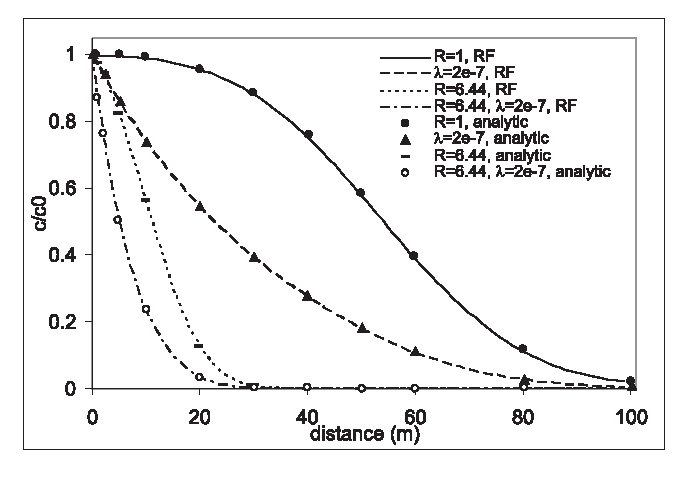
\includegraphics[width=0.8\textwidth]{PART_II/C/fig59.eps}
\caption{Concentration distributions of the four components after 100~d}
\label{fig59}
\end{figure}
